% This must be in the first 5 lines to tell arXiv to use pdfLaTeX, which is strongly recommended.
%\pdfoutput=1ex
% In particular, the hyperref package requires pdfLaTeX in order to break URLs across lines.

\documentclass[11pt]{article}

% Remove the "review" option to generate the final version.
\usepackage{ACL2023}
\usepackage{graphicx}
\usepackage{float}


% Standard package includes
\usepackage{times}
\usepackage{latexsym}

% For proper rendering and hyphenation of words containing Latin characters (including in bib files)
\usepackage[T1]{fontenc}
% This assumes your files are encoded as UTF8
\usepackage[utf8]{inputenc}

% This is not strictly necessary, and may be commented out.
% However, it will improve the layout of the manuscript,
% and will typically save some space.
\usepackage{microtype}

% This is also not strictly necessary, and may be commented out.
% However, it will improve the aesthetics of text in
% the typewriter font.
\usepackage{inconsolata}

\title{Branching Out: NLP Plant Recommender}

\author{
Shubham Banavalikar \quad Ben Robbins \quad Najmeh Rahimi \\
W266: Natural Language Processing \\
UC Berkeley School of Information \\
\texttt{\{nina, ali, mo\}@ischool.berkeley.edu}
}

\begin{document}
\maketitle

\begin{abstract}
Plant identification is typically approached through images, yet many real-world botanical records and user queries are text-based. We develop an NLP system that predicts plant species from free-text descriptions and compare three model families: TF-IDF retrieval, Sentence-BERT embeddings with cosine similarity, and a domain-adapted BERT model fine-tuned on botanical text. Using ~3,000 curated plant entries from the Perenual API for training and independent Wikipedia descriptions for evaluation, we assess each model’s ability to capture botanical terminology and generalize across domains. We imagine a system where a user can describe their perfect garden plant and our system would be able to identify the plant closest to what they are describing. Evaluation is done by generating a user's potential description using ChatGPT and the wikipedia entry for each plant. We then see if our models are able to pick out the plant based on the generated query as the top result or in the top 5 and 10. Our results improved upon the base line TF-IDF (0.129 top 10 accuracy) with our domain-adapted BERT model achieving a top 10 accuracy of around 0.190 and the Sentence-BERT embedding model around 0.202. This leaves major room for improvement as the accuracy.
\end{abstract}

\section{Introduction}

Text-based plant identification is a challenging and understudied problem. While most consumer and scientific plant identification systems rely on images, many real-world scenarios involve only textual descriptions. Botanists record species traits in field notebooks; gardeners describe the type of plant they want without having a photo; and online plant databases contain rich textual descriptions of morphology, habitat, and care requirements. Enabling a model to infer a plant species directly from such descriptions would provide a practical tool for classification, recommendation, and knowledge retrieval.
This project aims to build a model that takes free-text plant descriptions and predicts the most likely species based on a user's description of the plant they want. Compared to standard NLP tasks, this domain presents several challenges such as a high variability in text form (expert botanical descriptions vs. casual garden language), domain-specific terminology (e.g., lanceolate, pinnate, glabrous, deciduous), sparse/vague descriptions, and cross-domain robustness as models must generalize beyond the style of their training data. To turn this task into a well-structured experiment, we define the central research question:

\begin{quote}
\textbf{Does a domain-fine-tuned BERT encoder outperform SBERT and classical retrieval for predicting plant species from free-text descriptions?}
\end{quote}

\section{Project Overview}

\subsection{Datasets Used}

We initially explored recreating the dataset in
\cite{domazetoski2025planttraits},
which relies on species descriptions scraped from the Plants of the World Online (POWO)
database. However, this dataset was not publicly released, and reproducing it required
extensive web scraping and preprocessing to resolve inconsistencies in formatting, missing
fields, and taxonomic structure. Because reconstructing a reliable version of this dataset
was beyond the scope of our project timeline, we transitioned to an alternative public source.

Our final training dataset was built using the Perenual Botanical API
\cite{perenualAPI}, from which we extracted 3{,}000 plant entries.
Each entry includes structured horticultural attributes (e.g., sunlight requirements,
watering needs, soil type, growth cycle) as well as a free-text description of the species.
The raw dataset contained 1{,}548 unique common names and 3{,}000 unique scientific names.
Since users of a plant recommendation or identification system are more likely to interact
using common names rather than scientific nomenclature, we selected \textbf{common names
as the prediction labels} for all retrieval-based models.

To evaluate cross-domain generalization, we constructed an independent validation set
consisting of Wikipedia-derived plant descriptions. These descriptions differ substantially
in writing style and lexical choice from the Perenual dataset, allowing us to test model
robustness under more natural and diverse input conditions.

\subsection{Background}

Domazetoski et al.~ \cite{domazetoski2025planttraits} demonstrated that transformer-based models can extract
functional plant traits from long botanical descriptions, highlighting the importance
of domain-specific vocabulary adaptation for improving model performance. Their findings
motivate our hypothesis that fine-tuning BERT on botanical text will outperform general
pretrained models for species identification.

Several related works examine recommendation and retrieval using item descriptions.
RecoBERT \cite{ecommerceNLP2021} introduces domain-adapted encoders for catalog item retrieval
and shows that fine-tuned BERT models yield substantial improvements in domain-specific
semantic understanding.

Across all cited literature, no prior study evaluates species prediction directly from
textual plant descriptions as a classification or ranking task. Existing research focuses
on trait extraction, embedding analysis, or general recommender systems---not on
identifying plant species from free-text descriptions. This project addresses that gap.

\subsection{Data Representation and Preprocessing}

The Perenual API returns plant information in a nested JSON format containing a mix
of free-text descriptions, categorical attributes (e.g., sunlight level, watering
frequency, growth cycle), and boolean variables (e.g., drought tolerant, poisonous
to pets). To facilitate model training, we flattened the JSON structure into a tabular
CSV file in which each row corresponds to a single plant. The resulting dataset
includes both the original description field and a variety of structured metadata
capturing morphological, ecological, and horticultural properties.

Although ten plants in the dataset lacked a description field, we retained them
because the remaining attributes still contain meaningful biological information.
To convert the full set of structured attributes into a form suitable for NLP models,
we developed two text-construction pipelines.

In the first approach, we transformed all categorical and boolean fields into
human-readable phrases and concatenated them with the original description. This
flattened textual representation allowed TF--IDF and transformer-based encoders to
consume a unified text field that incorporates both free-text and structured data.

In the second approach, we used a large language model (ChatGPT) to generate a
natural-sounding sentence-level summary for each plant. The model received all
available structured fields and produced a coherent paragraph describing morphology,
growth requirements, and ecological traits. These generated descriptions served as
alternative inputs for evaluating whether LLM-based text synthesis improves retrieval
performance compared to rule-based text construction.

Together, these two representations enabled us to investigate how different text
formats influence downstream species identification models.

\begin{figure*}[h!]
    \centering
    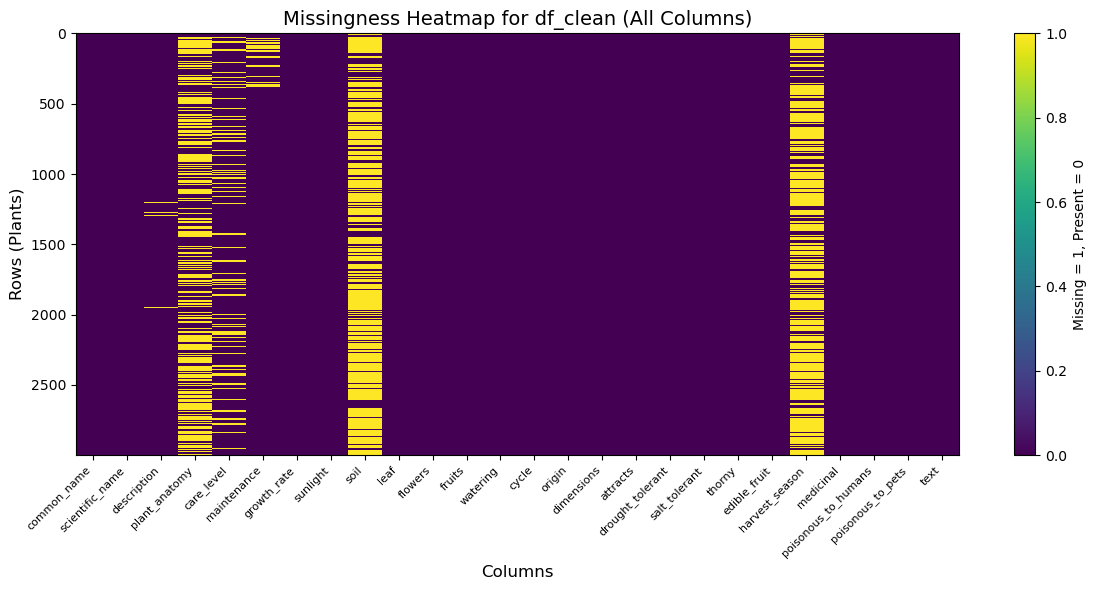
\includegraphics[width=\textwidth]{missing_data.png}
    \caption{Visualization of missing values across plant attributes in the Perenual dataset.}
    \label{fig:missing-data}
\end{figure*}

\section{Models}

We evaluate three retrieval-based models for text-only plant species identification:
a TF--IDF baseline, a domain-adapted BERT model (RecoBERT), and an advanced
Sentence-BERT encoder. Each model is trained on two versions of the Perenual dataset:
(1) a rule-based ``flattened'' text representation constructed from structured
attributes, and (2) an LLM-generated natural-language description synthesized from
the same attributes. This allows us to measure not only model quality but also the
impact of different text-construction approaches on retrieval accuracy. All models
are evaluated on an external validation set derived from Wikipedia plant descriptions,
and we report Top-1 and Top-10 accuracy to capture both strict and lenient retrieval
performance.

\subsection{Baseline Model}

As a classical baseline, we implemented a TF--IDF retrieval model that treats plant
identification as a text-matching problem rather than a supervised classifier. Each
plant entry in the training set was converted into a single enriched text document
combining its natural-language description with structured attributes (sunlight,
soil, watering, morphology, boolean traits, etc.). We applied scikit-learn's
\texttt{TfidfVectorizer} using unigrams and bigrams to capture both individual
botanical terms and short phrases. Test descriptions were vectorized using the same
vocabulary, and species predictions were obtained by computing cosine similarity
between each query vector and the full set of training vectors. The model returns
the most similar species (Top-1) or the top-$K$ most similar candidates, providing
a simple and interpretable keyword-based baseline against which the embedding-based
models can be compared.

\subsection{Reco BERT}

RecoBERT has 2 components: title-description model and masked-language model. The
title-description model's objective is to learn whether or not a given plant name
and plant description are related. In the paper, they pass tokenized titles and
descriptions (with some masked tokens) through BertModel, average the title
and description embeddings separately, and compute cosine similarities between the
averages. The loss function is defined to optimize for higher cosine similarity
between related plant names and descriptions. We also attempted a variation of this
where instead of using the embedding averages, we took the pooler_output parts of
the BertModel title and description outputs and computed their cosine similarities.
The masked-language model's objective is to learn embeddings for masked tokens that
give high weight to the original token. This allows for incorporating domain-specific
nuances. Specifically, it projects BertModel embeddings onto the dimension of vocabulary
size and uses a loss function that optimizes for a high embedding value for the index
corresponding to the original token.

\subsection{Advance Sentence BERT}

For the implementation of SBert we first used all-MiniLM-L6-v2 from hugging face to encode both the Perenual data and the text generated from the wikipedia descriptions. For each Perenual description embedding a cosine similarity was run against each of the generated descriptions. Then the top k similar embeddings were selected for each Perenual description where k = 1, 5, and 10. Each of these embeddings were then translated back into their plant names. Accuracy was calculated for each of the k values where the original Perenual name was in the list of predicted values.

In an attempt to improve the accuracy the same model was then finetuned. For this all but the last layer of the model had their parameters frozen. The Perenual dataset text descriptions with the description generated from ChatGPT based on the Perenual dataset were paired with a cosine similarity of 1. To generate some negative examples the descriptions were shifted 5 places. These were given a cosine similarity of 0. The model was then finetuned over one epoch using the CoSENTLoss loss function with a batch size of 16 and a warm up ratio of 0.1.
Code: \href{https://github.com/NajmeRah/DATASCI266_FinalProject/blob/main/Code/SBert.ipynb}{SBERT Code}

\section{Results}


\subsection{Accuracy}

\begin{table}[H]
\centering
\begin{tabular}{lccc}
\hline
\textbf{Model 1} & \textbf{Top-1 Acc} & \textbf{Top-5 Acc} & \textbf{Top-10 Acc} \\
\hline
TF--IDF         & 0.003 & 0.019 & 0.042 \\
RecoBERT        & 0.010 & 0.050 & 0.130 \\
Sentence-BERT   & 0.051 & 0.133 & 0.188 \\
\hline
\end{tabular}
\caption{Retrieval accuracy on the Wikipedia evaluation set using
ChatGPT-generated descriptions as the training representation.}
\label{tab:results-llm}
\end{table}

\begin{table}[H]
\centering
\begin{tabular}{lccc}
\hline
\textbf{Model 2} & \textbf{Top-1 Acc} & \textbf{Top-5 Acc} & \textbf{Top-10 Acc} \\
\hline
TF--IDF         & 0.033 & 0.085 & 0.129 \\
RecoBERT        & 0.010 & 0.090 & 0.190 \\
Sentence-BERT   & 0.050 & 0.141 & 0.202 \\
\hline
\end{tabular}
\caption{Retrieval accuracy on the Wikipedia evaluation set using the
rule-based flattened \texttt{text} representation of the Perenual data.}
\label{tab:results-flat}
\end{table}



% TODO: add your TF-IDF / RecoBERT / SBERT accuracy numbers

\subsection{Comparison of Results}

% TODO: short discussion comparing models and text representations

\section{Limitations}

% TODO: brief limitations paragraph

\section*{Ethics Statement}

% TODO: short ethics statement if required

\bibliographystyle{acl_natbib}
\bibliography{custom}

\end{document}
